\textbf{(Numerical Comparison.)} For Euler's Method, the Trapezoidal
Rule, Simpson's Rule, and the standard $4$-th order Runge-Kutta
Method solve the initial value problem
\begin{align}
y^\prime &= y \\
y(0) = 1\\
x \in [0,1]
\end{align}
with step-sizes $h = 2^{-s}$ where $s = 3,4,\dots,15$. Plot the error
at the right end-point, i.e. $y(1) - y_n$ (where $n = 1/h$), against
$h$. You may wish to superimpose the plots. If you like use
appropriate logarithmic graph paper. Comment on your results. (For
Simpson's rule use the exact starting value $y_1 = y(h)$.) Send me
your program by e-mail.

The ``standard'' Runge-Kutta method is:
\[
y_{n+1} = y_n + \frac{h}{6} (K_1 + 2K_2 + 2K_3 + K_4)
\]
where
\begin{align*}
K_1 &= f(x_n, y_n) \\
K_2 &= f \left(x_n + \frac{h}{2}, y_n + \frac{h}{2} K_1 \right) \\
K_3 &= f \left(x_n + \frac{h}{2}, y_n + \frac{h}{2} K_2 \right) \\
K_4 &= f \left(x_n + h, y_n + h K_3 \right) \\
\end{align*}

{\color{blue}

First we define a general method for iteration. Our iteration method
takes a function of the form $y^\prime(x,y)$, and in our case we just
return $y$. Next we define a list of the step sizes we would like to
compare against.

\begin{minted}[mathescape,
               linenos,
               numbersep=5pt,
               gobble=0,
               frame=lines,
               framesep=2mm]{clojure}
(defn lmm-ode-solve [f init & {:keys [x-max h method]}]
  {:pre [x-max h method]}
  (take-while #(<= (first %) x-max)
              (iterate (method f h)
                       init)))

(def y' (fn [x y] y))
(def s (range 3 16))
(def h (map #(Math/pow 2 (- %)) s))
\end{minted}

Each method function returns a method that can be iterated on. This
lets us encapsulate the original ODE, and step size. We return a
vector with $[x, y]$ values so that the next iteration can make use of
both. The final result is a list of coordinate pairs which we can plot
or use to measure error. We will use \texttt{map} to run this on all
of our step sizes.

\begin{enumerate}[leftmargin=0pt]
  %\setlength{\leftmargin}{0pt}

\item \textbf{Euler's Method}
\begin{align}
  y_{n+1} - y_n = h f_n
\end{align}

\begin{minted}[mathescape,
               linenos,
               numbersep=5pt,
               gobble=0,
               frame=lines,
               framesep=2mm]{clojure}
(defn eulers [f h]
  (fn [[x y]]
    [(+ x h)
     (+ y (* h (f x y)))]))

(def euler-results (map #(lmm-ode-solve y'
                                        [0 1]
                                        :x-max 1
                                        :h %
                                        :method eulers)
                        h))
\end{minted}



\item \textbf{Trapezoidal Rule}
\begin{align}
  y_{n+1}- y_n = \frac{h}{2} (f_{n+1} + f_n)
\end{align}

\begin{minted}[mathescape,
               linenos,
               numbersep=5pt,
               gobble=0,
               frame=lines,
               framesep=2mm]{clojure}
(defn trapezoidal-rule [f h]
  (fn [[x y]]
    (let [K1 (* h (f x y))
          K2 (* h (f (+ x h) (+ y K1)))]
      [(+ x h)
       (+ y (* 1/2 (+ K1 K2)))])))

(def trapezoid-results (map #(lmm-ode-solve y'
                                            [0 1]
                                            :x-max 1
                                            :h %
                                            :method trapezoidal-rule)
                            h))
\end{minted}

\item \textbf{Simpons's Rule}
\begin{align}
  y_{n+2} - y_n = \frac{h}{3} (f_{n+2} + 4 f_{n+1} + f_n)
\end{align}

\begin{minted}[mathescape,
               linenos,
               numbersep=5pt,
               gobble=0,
               frame=lines,
               framesep=2mm]{clojure}
(defn simpsons-rule [f h]
  (fn [[x y]]
    (let [K1 (* h (f x y))
          K2 (* h (f (+ x (/ h 2)) (+ y K1)))
          K3 (* h (f (+ x h) (+ y K2)))]
      [(+ x (* h 2))
       (+ y (* 1/3 (+ K1 (* 4 K2) K3)))])))

(def simpsons-results (map #(lmm-ode-solve y'
                                           [0 1]
                                           :x-max 1
                                           :h %
                                           :method simpsons-rule)
                           h))
\end{minted}

\item \textbf{Runge Kutta:}

\begin{minted}[mathescape,
               linenos,
               numbersep=5pt,
               gobble=0,
               frame=lines,
               framesep=2mm]{clojure}
(defn runge-kutta-4 [f h]
  (fn [[x y]]
    (let [K1 (* h (f x y))
          K2 (* h (f (+ x (/ h 2)) (+ y (/ K1 2))))
          K3 (* h (f (+ x (/ h 2)) (+ y (/ K2 2))))
          K4 (* h (f (+ x h) (+ y K1)))]
      [(+ x h)
       (+ y (* 1/6 (+ K1 (* 2 K2) (* 2 K3) K4)))])))

(def runge-results (map #(lmm-ode-solve y'
                                        [0 1]
                                        :x-max 1
                                        :h %
                                        :method runge-kutta-4)
                        h))
\end{minted}

\end{enumerate}

Lastly we can compute the error values and plot them.

\begin{minted}[mathescape,
               linenos,
               numbersep=5pt,
               gobble=0,
               frame=lines,
               framesep=2mm]{clojure}
(defn errors [results]
  (map #(Math/abs (- (y 1) (last (last %))))
       results))

(def euler-errors (errors euler-results))
(def trapezoid-errors (errors trapezoid-results))
(def simpsons-errors (errors simpsons-results))
(def runge-errors (errors runge-results))
\end{minted}

\begin{figure}[H]
\centering
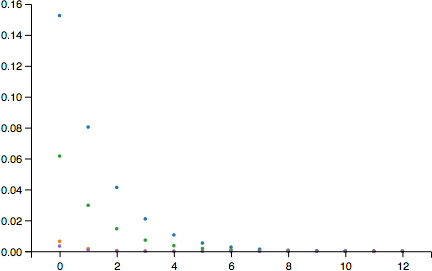
\includegraphics[scale=0.65]{numerical-comparison-errors.png}
\caption{Error for each value of $h$. The indices of the $x$-axis are
shifted: $0$ is for $h = 2^{-3}$, $1$ for $h = 2^{-4}$, $\dots$. Blue
is Euler's method, orange is the trapezoid rule, green is Simpson's
Rule, and purple is the Runge Kutta method.}
\end{figure}

We can see that each method performs differently, but that they all
achieve more accuracy with a smaller step size. In particular the
Runge-Kutta method and the trapezoid rule are very effective.

}
